\documentclass[a4paper,10pt]{article}
\usepackage{listings}
\usepackage{color}
\usepackage{graphicx}
\usepackage{textcomp}

\lstset{language=Java}
\lstset{breaklines=true, numbers=left}
\lstset{tabsize=4}

\definecolor{CommentColor}{rgb}{0,0.5,0} 
\definecolor{KeywordColor}{rgb}{0,0,0.5}

\lstset{commentstyle=\scriptsize\color{CommentColor}\itshape}
\lstset{keywordstyle=\scriptsize\color{KeywordColor}\bfseries}
\lstset{basicstyle=\scriptsize}
\lstset{identifierstyle=\scriptsize}
\lstset{stringstyle=\scriptsize}

% \lstset{basicstyle=\ttfamily}

\definecolor{lightblue}{rgb}{0.7,0.7,1}
\definecolor{lightyellow}{rgb}{1,1,0.5}
\definecolor{lightred}{rgb}{1,0.5,0.5}
\definecolor{lightgreen}{rgb}{0.7,1,0.7}

\newcommand{\src}[1]{\texttt{#1}}

\newcommand{\property}[4]{\item[#1] \mbox{ } \begin{description} \item[Type] \src{#2} \item[Default] #3 \item[Usage] #4  \end{description}}

% thanks to http://www.alfredklomp.com/programming/tex/macros/
\long\def\greybox#1#2#3{%
    \newbox\contentbox%
    \newbox\bkgdbox%
    \setbox\contentbox\hbox to \hsize{%
        \vtop{
            \kern\columnsep
            \hbox to \hsize{%
                \kern\columnsep%
                \advance\hsize by -2\columnsep%
                \parbox{0.1\hsize}{\includegraphics[width=\hsize]{#2}}%
                \hspace{0.025\hsize}%
                \advance\hsize by -0.125\hsize%
                \setlength{\textwidth}{\hsize}%
                \vbox{
                    \parskip=\baselineskip
                    \parindent=0bp
                    \parbox[c]{\hsize}{#3}
                }%
                \kern\columnsep%
            }%
            \kern\columnsep%
        }%
    }%
    \setbox\bkgdbox\vbox{
	\color{#1}
        \hrule width  \wd\contentbox %
               height \ht\contentbox %
               depth  \dp\contentbox
	\color{black}
    }%
    \wd\bkgdbox=0bp%
    \vbox{\hbox to \hsize{\box\bkgdbox\box\contentbox}}%
    \vskip\baselineskip%
}

\newcommand{\designbox}[1]{\greybox{lightgreen}{design}{#1}}
\newcommand{\classbox}[1]{\greybox{lightyellow}{class}{#1}}
\newcommand{\warningbox}[1]{\greybox{lightred}{stop}{#1}}
\newcommand{\infobox}[1]{\greybox{lightblue}{info}{#1}}

\title{DockingFrames 1.0.7 - Common}
\author{Benjamin Sigg}

\begin{document}

\maketitle
\newpage

\tableofcontents
\newpage

\section{Introduction}

\src{DockingFrames} is an open source Java Swing framework. This framework allows to write applications with floating panels. A floating panel is a \src{Component} that can be moved around by the user.

\src{DockingFrames} consists of two libraries, \src{Core} and \src{Common}. \src{Common} provides advanced functionalities that are built on top of \src{Core}. \src{Common} is a wrapper around \src{Core} and requires \src{Core} to work.

This document covers only \src{Common}, \src{Core} has its own guide. Not all the details of \src{Common} are described, but this document gives a nice oversight of the more important aspects.

You can utilize \src{Common} without understanding \src{Core}. But knowing at least some basics about \src{Core} will make life much easier.

\section{Notation}
This document uses various notations.

Any element that can be source code (e.g. a class name) and project names are written mono-spaced like this: \src{java.lang.String}. The package of classes and interfaces is rarely given since almost no name is used twice. The packages can be easily found with the help of the generated API documentation (\src{JavaDoc}).

\infobox{Tips and tricks are listed in boxes.}

\warningbox{Important notes and warnings are listed in boxes like this one.}

\classbox{Implementation details, especially lists of class names, are written in boxes like this.}

\designbox{These boxes explain \textit{why} some thing was designed the way it is. This might either contain some bit of history or an explanation why some awkward design is not as bad as it first looks.}

\section{Basics}
\src{Common} is partitioned into three sub-projects.

For clients the sub-project \src{common} is the most interesting. This project is the main layer above \src{Core} and also the most advanced layer in the whole framework.

The sub-project \src{facile} builds a basis for the features of \src{common}. In theory \src{facile} could be used without \src{common} but in practice the classes and interfaces are clearly designed to be used by or together with \src{common}.

Finally \src{support} consists of classes that are just used by \src{facile} and \src{common}. These classes have few to none relations with \src{DockingFrames} and can be used alone as well.

\subsection{Concepts}
In the understanding of \src{Common} an application consists of one main-window and maybe several supportive frames and dialogs. The main-window is most times a \src{JFrame} and the application runs as long as this frame is visible. The main-window consists of several panels. Each panel shows some part of the data. E.g. the panels of a browser could be the ``history'', the ``bookmarks'' and the open websites.

\src{Common} is an additional layer between panels and main-frame. It separates them and allows the user to drag \& drop panels.

To do so each panel gets wrapped into a \src{CDockable}. These \src{CDockable}s are then put onto \src{CStation}s. A controller (\src{CControl}) handles the movement of the dockables.

\begin{figure}[ht]
\centering
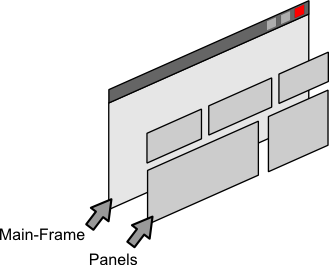
\includegraphics[scale=1]{app_without}
\caption{The standard application without \src{Common}. A main-frame and some panels that are put onto the main-frame.}
\label{fig:app_without}
\end{figure}

\begin{figure}[ht]
\centering
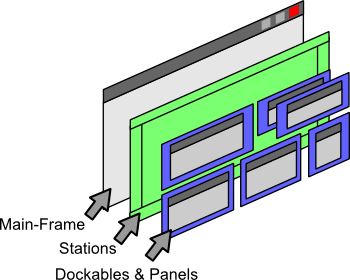
\includegraphics[scale=1]{app_with}
\caption{An application with \src{Common}. The panels are wrapped into dockables. The dockables are put onto stations which lay on the main-frame. Dockables can be moved to different stations.}
\label{fig:app_with}
\end{figure}

\subsection{Hello World}
This chapter introduces the very basic vocabulary and shows a first example. In depth discussions of the concepts and implementations follow in the chapters afterwards.

\subsubsection{Setup controller}
The first step should be to create a \src{CControl}. \src{CControl} has more than one constructor, for this example it is sufficient to use the one constructor which requires only a \src{JFrame}. \src{CControl} monitors the state of this frame and ensures that the windows of \src{Common} are only visible when the frame is visible. Also dialogs created by the framework will have this frame as parent.

The code to create the controller looks like this:
\begin{lstlisting}
public class Example{
	public static void main( String[] args ){
		JFrame frame = new JFrame();
		frame.setDefaultCloseOperation( JFrame.EXIT_ON_CLOSE );
		
		CControl control = new CControl( frame );
		
		...
\end{lstlisting}

\subsubsection{Setup stations}
The second step is to setup the layer between main-frame and dockables. There are different \src{CStation}s available. For example the \src{CMinimizeArea} shows minimized \src{CDockable}s. Instead of creating the stations manually one can also use a \src{CContentArea}. The \src{CContentArea} is a panel that consists of five stations. In the center a grid of dockables is shown, at the border four areas are reserved for minimized dockables.

There is always a default-\src{CContentArea} available, it can be accessed by calling \src{getContentArea} of \src{CControl}. If required additional \src{CContentArea}s can be created by the method \src{createContentArea} of \src{CControl}.

A \src{CContentArea} is a \src{JComponent}, so its usage is straight forward. Line \src{10} is the important new line in this code:
\begin{lstlisting}
public class Example{
	public static void main( String[] args ){
		JFrame frame = new JFrame();
		
		frame.setDefaultCloseOperation( JFrame.EXIT_ON_CLOSE );
		
		CControl control = new CControl( frame );
		
		frame.setLayout( new GridLayout( 1, 1 ) );
		frame.add( control.getContentArea() );
		
		...
\end{lstlisting}

\infobox{\src{CControl} always creates an additional station for handling externalized dockables.}

\subsubsection{Setup dockables}
A \src{CDockable} is the thing that can be dragged and dropped by the user. A \src{CDockable} has a set of properties, e.g. what text to show as title, whether it can be maximized, what font to use when focused, and so on.
\src{CDockable}s are divided into two categories: ``single'' and ``multi'' dockables. These categories are explained later, for this first example single dockables are the correct choice. Single dockables are represented by the interface \src{SingleCDockable}. The class \src{DefaultSingleCDockable} provides an easy to use implementation.
In the code below new single dockables are created in lines \src{23-25} and \src{43-48}. They need to be registered at the \src{CControl} in lines \src{27-29}, otherwise they cannot be shown. Optionally the initial position can be set like in line \src{33} and \src{36}. There is no need to set the position of the first dockable \src{red}: since it is the first it gets per default all the space.

\begin{lstlisting}
import java.awt.Color;
import java.awt.GridLayout;

import javax.swing.JFrame;
import javax.swing.JPanel;

import bibliothek.gui.dock.common.CControl;
import bibliothek.gui.dock.common.CLocation;
import bibliothek.gui.dock.common.DefaultSingleCDockable;
import bibliothek.gui.dock.common.SingleCDockable;

public class Example{
	public static void main( String[] args ){
		JFrame frame = new JFrame();
		
		frame.setDefaultCloseOperation( JFrame.EXIT_ON_CLOSE );
		
		CControl control = new CControl( frame );
		
		frame.setLayout( new GridLayout( 1, 1 ) );
		frame.add( control.getContentArea() );
		
		SingleCDockable red = create( "Red", Color.RED );
		SingleCDockable green = create( "Green", Color.GREEN );
		SingleCDockable blue = create( "Blue", Color.BLUE );
		
		control.add( red );
		control.add( green );
		control.add( blue );
		
		red.setVisible( true );
		
		green.setLocation( CLocation.base().normalSouth( 0.4 ));
		green.setVisible( true );
		
		blue.setLocation( CLocation.base().normalEast( 0.3 ) );
		blue.setVisible( true );
		
		frame.setBounds( 20, 20, 400, 400 );
		frame.setVisible( true );
	}
	
	public static SingleCDockable create( String title, Color color ){
		JPanel background = new JPanel();
		background.setOpaque( true );
		background.setBackground( color );
		
		return new DefaultSingleCDockable( title, title, background );
	}
}

\end{lstlisting}

\section{Foundation}
This chapter focuses on the foundation of \src{Common}: \src{CControl}, the stations and dockables.

\subsection{Dockables}
As mentioned in the previous chapter \src{CDockable}s fall in one of two categories: ``single'' or ``multiple''. Only one instance of a single dockable may exist during runtime, but many (or none) instance of a multiple dockable may exist. In many cases both kind of dockables have the same behavior, but there are some exceptions when it comes to the storage of their location.

Every \src{CDockable} needs to be registered at a \src{CControl}, the methods with name \src{add} can be used. They need to be made visible by calling \src{setVisible} of \src{CDockable}.

\designbox{The interface \src{CDockable} has some awkward methods whose implementation is already described in the documentation. \src{CDockable} is not intended to be implemented by clients, but to be used by them. There is a subclass \src{AbstractCDockable} which provides the correct implementation for these awkward methods. Even in the framework itself no class (except \src{AbstractCDockable}) implements \src{CDockable} directly. The only reason for the existence of \src{CDockable} is to provide an abstraction from the implementation.}

\infobox{A \src{CDockable} is not a \src{Dockable}, but internally references a \src{Dockable}. This \src{Dockable} is always of type \src{CommonDockable}. It can be accessed through the method \src{intern} of \src{CDockable}. Clients should avoid modifying this \src{Dockable} directly.}

\subsubsection{SingleCDockable}
The representation of a single dockable is \src{SingleCDockable}. A single dockable is created once, added to the control and made visible. It remains in memory until explicitly removed from the \src{CControl} or the application terminates.

In order to store attributes (like the position) persistently each \linebreak \src{SingleCDockable} requires a unique identifier.

Clients best use a \src{DefaultSingleCDockable}. A \src{DefaultSingleCDockable} can be used like a \src{JFrame}, for example it also has a content-pane, has methods to set the title-text, etc.

Examples for single dockables could be:
\begin{itemize}
  \item A browser has one panel ``history'', the panel is shown on a single dockable.
  \item A view that is most of the time invisible. A single dockable is created lazily the first time when the view is shown.
\end{itemize}

\subsubsection{MultipleCDockable}
\src{MultipleCDockable} are used if the number of instances is not known prior to runtime. Each kind of \src{MultipleCDockable} is associated with a \linebreak \src{MultipleCDockableFactory}. The framework can delete or create new instances of this kind of dockable whenever they are needed.

Clients are required to install the \src{MultipleCDockableFactory} before using any \src{MultipleCDockable}. There is a class \src{DefaultMultipleCDockable} which should provide all the features a client needs.

An example:
\begin{lstlisting}
CControl control = ...

MultipleCDockableFactory<MyDockable, MyLayoutInformation> = new ...
control.addMultipleDockableFactory( "unique id", factory );

MyDockable dockable = new ...
control.add( dockable );
\end{lstlisting}
Notice that in line \src{4} a unique identifier needs to be assigned to the factory.

Implementing a \src{MultipleCDockableFactory} is easy. There is a method to read and to write meta-information from or to a \src{MultipleCDockable}. Meta-information itself is a \src{MultipleCDockableLayout} which has methods to write or read its content to a stream (e.g. to file). There are no restrictions to what meta-information really is.

Examples for multiple dockables are:
\begin{itemize}
 \item A text-editor can show many documents at the same time. Each document is shown in its own dockable.
 \item A 3D modeling software allows to see the modeled object from different angles. Each camera is a dockable.
\end{itemize}

\infobox{In \src{Common} each \src{CDockable} requires to have a unique identifier. The framework will automatically create an identifier for \src{MultipleCDockable}s.}

\designbox{Why the distinction between single and multiple dockables? The algorithms to store and load the layout (place and size of dockables) can either use existing objects or create new dockables. Using existing objects is preferred because the overhead of creation can be - at least for complex views - high. Single and multiple \src{CDockable}s represent this gap.}

\subsubsection{Visibility}
A dockable is either visible or invisible. The user cannot interact with the dockable unless it is visible. There is more than one path to change visibility.

The direct approach is to call the method \src{setVisible} of \src{CDockable}. This method will show the dockable at its last known location.

A dockable is made visible implicitly if it is added to any station. This can happen if for example using a \src{CGrid} like explained in chapter \ref{sec:location}.

Finally the user can make a dockable invisible by clicking on its close-button. Every subclass of \src{DefaultCDockable} has the method \src{setCloseable} to change whether the user can click away the element.

Visibility can be monitored with a \src{CDockableStateListener}. Either for a single dockable by adding the listener directly to the dockable, or globally by adding the listener to \src{CControl}. An example:
\begin{lstlisting}
CDockable dockable = ...
		
dockable.addCDockableStateListener( new CDockableAdapter(){
  @Override
  public void visibilityChanged( CDockable dockable ){
    System.out.println( "Visibility changed to '" + 
                         dockable.isVisible() + "'" );
  }
});
\end{lstlisting}

 The default behavior of the close-action is to call \src{setVisible} with \src{visible} set to \src{false}, so overriding this method is an easy way to introduce some additional code that is executed directly before the dockable closes.

\classbox{The close-action can be replaced by calling \src{putAction} with the key \src{ACTION\_KEY\_CLOSE} of \src{CDockable}. The action can be replaced at any time. More about actions in chapter \ref{sec:action}.}

\infobox{If the method \src{setLocation} of \src{AbstractCDockable} is called before the dockable is made visible, then the dockable is made visible at the supplied location. More about locations in chapter \src{sec:location}.}

\subsubsection{Mode}
If a \src{CDockable} is visible then it always is in an extended-mode. The extended mode tells something about the behaviour of the dockable and where it is placed. There are four extended modes available:
\begin{description}
 \item[normalized] The normal state of a dockable. It is placed on the main-frame of the application, but only covers a fraction of the main-frame.
 \item[maximized] A maximized dockable takes all the space it gets and often covers other dockables.
 \item[minimized] A minimzed dockable is not directly visible. Only a button at one edge of the main-frame indicates the existance of the dockable. If the button is pressed then the dockable pops up. As soon as it loses focus it disapears again.
 \item[externalized] The dockable receives its own window. Per default the window is an undecorated \src{JDialog} and child of the main-frame.
\end{description}

Users can change the extended mode either by dragging the dockable to a new area, or by clicking some buttons that are visible in the title of each dockable.

Clients can access and change the extended mode by calling \linebreak \src{getExtendedMode} and \src{setExtendedMode} of \src{CControl}. A dockable has no extended mode if not visible. Furthermore clients can forbid a dockable to go into some extended modes. Methods like \src{setMaximizable} of \src{DefaultCDockable} allow that. Finally clients can exchange the button that must be pressed by the user by calling \src{putAction} of \src{AbstractCDockable}. Keys for \src{putAction} are declared as \src{String} constants in \src{CDockable} with names like \src{ACTION\_KEY\_MINIMIZE}.

\subsection{Stations}
Stations are needed to place and show \src{CDockable}s. A station provides the \src{Component}(s) (e.g. a \src{JPanel} or a dialog) that are the parents of the dockables. Stations are represented through the interface \src{CStation}.

\src{CStation}s delegate most of their work to some \src{DockStation} of \src{Core}. Like dockables a \src{CStation} requires a unique identifier. This identifier is used to persistently store and load layout information.

\warningbox{Currently only the existing \src{DockStation}s from \src{Core} are truly supported by \src{Common}. The \src{StateManager} makes a few assumptions what station is associated with what mode, e.g. a \src{FlapDockStation} is associated with mode ``minimized''. Future versions of the framework might be designed more open, allowing developers to add new modes or other associations. Some improvements were already introduced in version 1.0.7.}

\subsubsection{All in one: CContentArea}
The preferred way to create stations is to use a \src{CContentArea}. A \src{CContentArea} is not a single \src{CStation} but a panel containing many stations. Each content-area has a center area where dockables are layed out in a grid, and four small areas at the border where dockables show up when they are minimized.

There is a default-\src{CContentArea} present and can be accessed through \linebreak \src{getContentArea} of \src{CControl}. A content-area can later be used like any other \src{Component}:
\begin{lstlisting}
JFrame frame = ...
CControl control = ...

CContentArea area = control.getContentArea();
frame.add( area );
\end{lstlisting}

If more than one content-area is needed then clients can use \linebreak \src{createContentArea} of \src{CControl} to create additional areas. These additional areas can later be removed through \src{removeContentArea}. The default content-area cannot be removed.

\infobox{The default content-area is create lazily. There is no obligation to use or create it, clients can as well directly call \src{createContentArea} or not use them at all.}

\warningbox{While \src{CContentArea} has a public constructor clients should prefer to use the factory method \src{createContentArea}. In future releases the constructor might be changed.}

To place dockables onto a content-area a \src{CGrid} can be of help. With the method \src{deploy} the content of a whole \src{CGrid} can be put onto the center area. More about \src{CGrid} and other mechanisms to position elements are listed up in chapter \ref{sec:location}.

\subsubsection{Center area: CGridArea}
A \src{CGridArea} is kind of a lightweight version of \src{CContentArea}. A grid-area contains normalized and maximized dockables. Other than a content-area it cannot show minimized dockables.

\src{CGridArea}s should be created through the factory method \src{createGridArea} of \src{CControl}. If it is no longer required it can be removed through the method \src{removeStation}.

Like \src{CContentArea} a \src{CGridArea} has the method \src{deploy} to add a whole set of dockables quickly to the area.

Usage of a grid-area could look like this:

\begin{lstlisting}
JFrame frame = ...
CControl control = ...

CGridArea center = control.createGridArea( "center" );
frame.add( center.getComponent() );
\end{lstlisting}
Notice that in line \src{5} the method \src{getComponent} has to be called. This method returns the \src{Component} on which the station lies.

\classbox{Some more things that might be interesting:
\begin{itemize}
\item A grid-area implements \src{SingleCDockable}, hence it can be a child of another area. Remember that the area must be manually added to the \src{CControl} as dockable.
\item The method \src{setMaximizingArea} influences of what happens when a child of the area gets maximized. If \src{true} was given to the method then the child gets maximized within the boundaries of the grid-area. Otherwise the child might cover the area or even be transfered to another area.
\end{itemize}}

\subsubsection{Minimized: CMinimizeArea}
Most things that were said for \src{CGridArea} hold true for \src{CMinimizeArea} as well. A minimize-area should be created through \src{createMinimizeArea} of \src{CControl}.

\subsubsection{Grouping Dockables: CWorkingArea}
The \src{CWorkingArea} is a subclass of \src{CGridArea}. The difference between them is, that the property \src{working-area} is \src{false} for a grid-area, but \src{true} for a \src{CWorkingArea}. 

Having this property set to \src{true} places some constraints on the station:
\begin{itemize}
\item Children of this station cannot be put moved to another station if that other station shows dockables in normalized mode. For a user this means that children can only be minimized, maximized or externalized, but not dragged away.
\item The user cannot drag dockables away from the station unless they are already children of the station.
\item If the station has no children then it appears as grey, empty space which does not go away.
\item Children of a working-area are not stored for temporary layout. For the user this means that applying a layout does neither affect the station, or dockables that can be put onto the station.
\end{itemize}

\src{CWorkingArea}s can be used to display a set documents. For example in an IDE (like \src{Eclipse} or \src{Netbeans}) each source file would get its own \src{CDockable} which then is put onto the working-area.

\infobox{The children of a \src{CWorkingArea} are often good candidates for being \src{MultipleCDockable}s.}

\section{Locations} \label{sec:location}
Location means position and size of a dockable. A location can be relative to some parent of a dockable or it can be fix.

\subsection{For a single dockable: CLocation}
The location of a single dockable is represented by a \src{CLocation}. The method \src{getBaseLocation} of \src{CDockable} gets the current location and the method \linebreak \src{setLocation} changes the current location.

Most subclasses of \src{CLocation} offer one or more methods to optain new locations. For example a \src{CGridAreaLocation} offers \src{north}. While \linebreak \src{CGridAreaLocation} represents just some \src{CGridArea}, the location optained through \src{north} represents the upper half of the grid-area. Clients can chain together method calls to create locations:
\begin{lstlisting}
CGridAreaLocation root = ...
CDockable dockable = ...
		
CLocation location = root.north( 0.5 ).west( 0.5 ).stack( 2 );
dockable.setLocation( location );
\end{lstlisting}
The chain of calls in line \src{4} creates a location pointing to the upper left quarter of some grid-area. Assuming there is a stack of dockables in that quarter, the location points to the third entry of that stack. In line \src{5} the location of \src{dockable} is set, the framework will try to set \src{dockable} at the exact location but cannot make any guarantees (e.g. if there is no stack in the upper left quarter, then framework cannot magically invent one).

To create a root-location clients can call one of the static factory methods of \src{CLocation} or directly instantiate the location. Calling the factory methods of \src{CLocation} is preferred.

Setting the location of a dockable \src{a} to the location of another dockable \src{b} will move away \src{a} from its position. As an example:
\begin{lstlisting}
CDockable a = ...
CDockable b = ...

CLocation location = a.getBaseLocation();
b.setLocation( location );
\end{lstlisting}

If \src{a} should remain at its place then the method \src{aside} of \src{CLocation} can create a location that is near to \src{a}, but not exactly \src{a}'s position:
\begin{lstlisting}[firstnumber=5]
b.setLocation( location.aside() );
\end{lstlisting}

\classbox{\src{CLocation} is a wrapper around \src{DockableProperty}. While each \src{DockableProperty} has its own API and concepts, \src{CLocation}s unify usage by providing the chain-concept. The chain-concept allows some typesafety and should reduce the amount of wrongly put together locations. }

\subsection{For a group of dockables: CGrid}
Sometimes it is necessary to set the position of several dockables at once. For example when the application starts up a default layout could be created. If dockables are minimized or externalized the position can simply be set with \src{CLocation}s. If dockables are shown normalized on a grid-area, a working-area, or the center of a \src{CContentArea} then things get more complex. Using \src{CLocation} would require a precise order in which to add the dockables, and some awkward coordinates to make sure they are shifted at the right place when more dockables become visible.

\src{CGrid} is a class that collects dockables and their boundaries. All this information can then be put onto a grid-like areas in one command. Furthermore a \src{CGrid} can also automatically register dockables at a \src{CControl}. An example:
\begin{lstlisting}
CControl control = ...

SingleCDockable single = new ...
MultipleCDockable multi = new ...

CGrid grid = new CGrid( control );

grid.add( 0, 0, 1, 1, single );
grid.add( 0, 1, 1, 2, multi );

CContentArea content = control.getContentArea();
content.deploy( grid );
\end{lstlisting}
The \src{CControl} created in line \src{6} will call the \src{add}-methods of \src{control} (line \src{1}) with any dockable that is given to it. In lines \src{8,9} two dockables are put onto the grid. The numbers are the boundaries of the dockables. In line \src{12} the contents of the grid are put onto \src{content}. The dockables \src{single} and \src{multi} will be arranged such that \src{multi} has twice the size of \src{single}.

Boundaries are relative to each other, there is no minimal or maximal value for a coordinate or size. \src{CGrid} is able to handle gaps and overlaps, but such defections might yield awkward layouts.

\warningbox{Make sure not to add a dockable twice to a \src{CControl}. If using a \src{CGrid} the \src{add} method of \src{CControl} must not be called. 

Also note that there is a second constructor for \src{CGrid} that does not have any argument. If that second constructor is used, then the \src{CGrid} will not add dockables to any \src{CControl}.}

\infobox{Dockables can also be grouped in a stack by \src{CGrid}. Any two dockables with the same boundaries are grouped. The \src{add} method uses a vararg-argument, more than just one dockable can be placed with the same boundaries this way.}

\classbox{Internally \src{CGrid} uses a \src{SplitDockGrid}. \src{SplitDockGrid} contains an algorithm that creates a \src{SplitDockTree}. This tree has dockables as leafs and relations between dockables are modeled as nodes. A \src{SplitDockTree} can be used by a \src{SplitDockStation} to build up its layout. }

\subsection{For all dockables: layout}
The ``layout'' is the set of all locations, even including invisible dockables. \src{CControl} supports the storage and replacement of layouts automatically. \linebreak Clients only need to provide some factories for their custom dockables. A layout does not have direct references to any dockable, it is completely independent of gui-components.

There are four important methods in \src{CControl} used to interact with layouts:
\begin{itemize}
 \item \src{save} - stores the current layout. The method requires a \src{String} argument that is used as key for the layout. If a key is alread used then the old layout gets replaced with the new one.
 \item \src{load} - is the counterpart to \src{save}. It loads a layout that was stored earlier.
 \item \src{delete} - deletes a layout.
 \item \src{layouts} - returns all the keys that are in use for layouts.
\end{itemize}

\infobox{The class \src{CLayoutChoiceMenuPiece} can build some \src{JMenuItem}s that allow the user to save, load and delete layouts at any time. More about \src{MenuPiece}s can be found in chapter \ref{sec:menus}.}

\designbox{Layouts are divided into two subsets: ``entry'' and ``full'' layouts. An entry-layout does not store the location of any dockable that is associated with a working-area. A full-layout stores all locations. The method \src{save} always uses entry-layouts and a full-layout is only used when the applications properties are stored persistantly in a file.

Working-areas are intended to show some documents that are only temporarely available. Assuming that each dockable on a working-area represents one such document it makes perfectly sense not to replace them just because the user chooses another layout. Changing them would mean to close some documents and load other documents, and that is certainly not the behaviour the user would expect.}

\warningbox{The client is responsible to store the contents of any single-dockable. }

\subsubsection{Persistant Storage}
\src{Common} uses a class called \src{ApplicationResourceManager} to store its properties. Among other things all layout information is stored in this resource-manager. Normally any information in the resource-manager gots lost once the application shuts down. But clients can tell the resource-manager to write its contents into a file. Either they call \src{getResources} of \src{CControl} and then one of the many methods that start with ``write'' or they use directly \src{CControl}. An example:
\begin{lstlisting}
File file = new File( "layout.data" );

// write properties		
control.write( file );

// read properties
control.read( file );
\end{lstlisting}

\subsubsection{Dealing with lazy creation and missing dockables}
While \src{MultipleCDockable}s are created only when they are needed, \src{Common} assumes that \src{SingleCDockable}s are always present. However this assumption would require to create components that might never be shown. In order to solve the problem \src{SingleCDockableBackupFactory} was introduced. If a missing single-dockable is required the factories method \src{createBackup} is called. Assuming the factory returns not \src{null} then the new dockable is properly added to \src{CControl} and made visible.

\src{SingleCDockableBackupFactory}s need to be registered at the \src{CControl} using the method \src{addSingleBackupFactory}. They can also be removed using the method \src{removeSingleBackupFactory}. 

\infobox{If a dockable is removed from a \src{CControl} then normally all its associated location information is deleted. If however a backup-factory with the same id as the dockables id is registered, then the location information remains. If another dockable with the same id is later registered, then this new dockable inherits all settings from the old one.}

\classbox{\src{CControl}s behavior for missing dockables can be fine tuned with a \src{MissingCDockableStrategy}.} 

\section{Actions} \label{sec:action}


\section{Menus} \label{sec:menus}

\section{Unused text}
\classbox{The parameters of different constructors of \src{CControl} are:
\begin{description}
 \item[JFrame frame] The main-frame of the application.
 \item[WindowProvider window] The main-window of the application. This window will be the parent of all dialogs that are created by the framework. It is possible to replace this window at any time, but already created dialogs will not be affected by the change.
 \item[boolean restrictedEnvironment] If set to \src{true} then some unsecure optimizations are disabled. This allows to use \src{CControl} for unsigned applets or webstart applications.
 \item[CControlFactory factory] A factory used to create some elements of \src{Common}.
\end{description}
}


\end{document}